\chapter{Mechanika kontinua}
\section{Úvod}
% !TeX root = skripta-konstitutivni-vztahy.tex
% !TeX lastmodified = 2006-11-04

\subsection{Einsteinovo sčítací pravidlo}\label{sec:einsteinovo-scitaci-pravidlo}
Einsteinovo sčítací pravidlo se používá pro zjednodušení obecných tenzorových zápisů. Vyskytuje-li se v~některém členu opakovaný index (tzv. sčítací index, v~našem případě index~$k$) pak se provádí sumace přes tento index. Např. obecný zápis \hyperref[sec:green-lagrange]{Green-Lagrangeova} tenzoru přetvoření ve tvaru
\begin{equation}
	E^L_{ij} = \frac{1}{2} \left[ \frac{\partial u_i}{X_j} + \frac{\partial u_j}{X_i} + \frac{\partial u_k}{X_j} \frac{\partial u_k}{X_i} \right]
\end{equation}
je třeba interpretovat následovně:
\begin{equation}
	E^L_{ij} = \frac{1}{2} \left[ \frac{\partial u_i}{X_j} + \frac{\partial u_j}{X_i} + \sum_{k=1}^3 \frac{\partial u_k}{X_j} \frac{\partial u_k}{X_i} \right]
\end{equation}

% !TeX root = skripta-konstitutivni-vztahy.tex
% !TeX lastmodified = 2016-10-18

\subsection{Shear}
Jak \uv{simple shear}, tak \uv{pure shear} je zvykem používat ve smyslu deformace. Oba stavy deformace jsou teoreticky ekvivalentní, v~praxi tomu však tak nemusí být (není snadné pro obecný Poissonův poměr $\mu$ realizovat příslušné stavy deformace, pro $\mu = \num{0.5}$ je to snazší).

\subsubsection{Simple shear}
\begin{figure}[H]
	\centering
	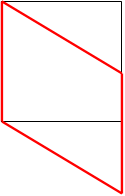
\includegraphics[height=4cm]{simple-shear}
	\caption{Simple shear}
	\label{fig:simple-shear}
\end{figure}

\begin{itemize}
	\item černá je nedeformovaná geometrie
	\item červená je deformovaná geometrie
	\item třetí rozměr zůstává bez změny ($\lambda_3 = 1$)
	\item volumetrická změna $= 0$
	\item pozor: indukují se i normálová napětí (při velkých -- \uv{neinfinitezimálních} -- deformacích)
	\item hlavní osy tenzoru deformace se v průběhu vzrůstající úrovně deformace NATÁČEJÍ
\end{itemize}

Praktická realizace:
\begin{figure}[H]
	\centering
	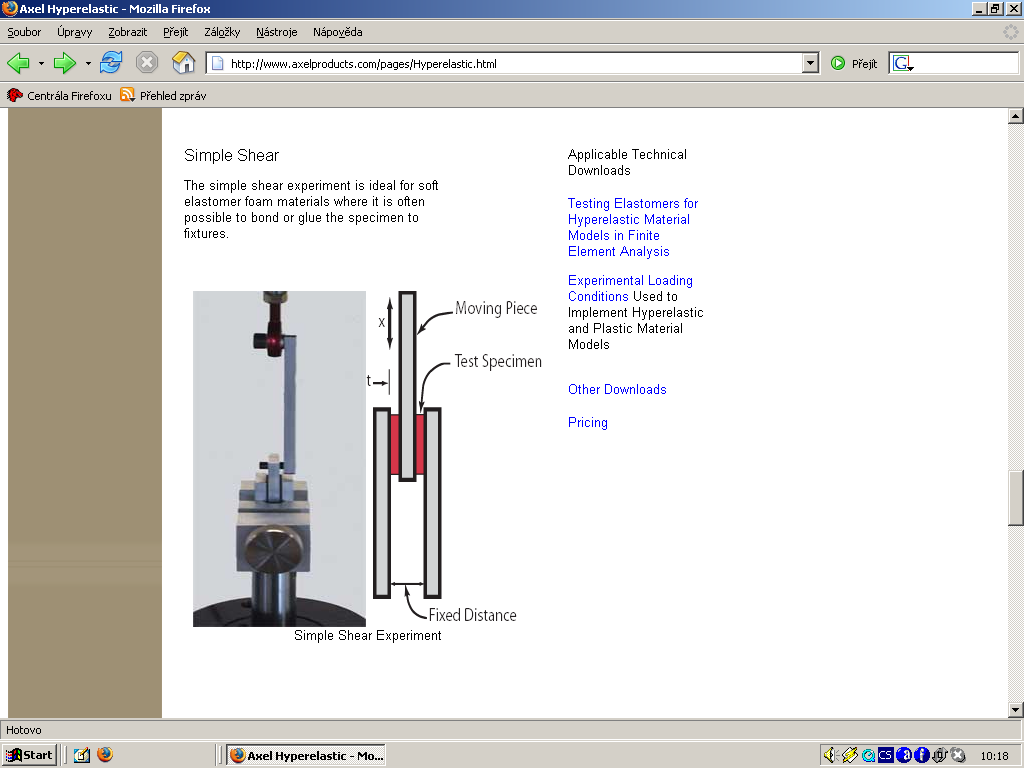
\includegraphics[width=0.4\linewidth]{Obrazky/simple-shear-experiment}
	\caption{Simple shear experiment}
	\label{fig:simple-shear-experiment}
\end{figure}

\subsubsection{Pure shear}
\begin{figure}[H]
	\centering
	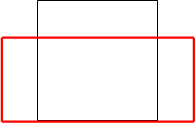
\includegraphics[height=4cm]{pure-shear}
	\caption{Pure shear}
	\label{fig:pure-shear}
\end{figure}

\begin{itemize}
	\item třetí rozměr zůstává bez změny ($\lambda_3 = 1$)
	\item volumetrická změna $= 0$ (v~praxi při tzv. \uv{pure shear} testu není většinou splněno)
	\item praktická realizace: tahem v~širokých čelistech na širokém vzorku nebo tlakem hranolového vzorku při zabránění jedné z~příčných deformací
\item hlavní osy deformace se v~průběhu vzrůstající úrovně deformace nenatáčí
\end{itemize}

\subsubsection{Vysvětlení vzájemné ekvivalence}
\begin{figure}[H]
	\centering
	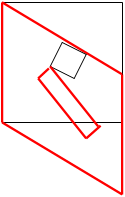
\includegraphics[height=4cm]{shear-vzajemna-ekvivalence}
	\caption{Vzajemná ekvivalence}
	\label{fig:shear-vzajemna-ekvivalence}
\end{figure}

Na případu „simple shear“ lze pro danou úroveň deformace (gama) vždy nalézt na deformovaném vzorku ortogonální (pravoúhlý) element, kterému v nedeformované konfiguraci odpovídá rovněž ortogonální element. Tedy na takovém elementu neproběhl smyk vůči jeho hranám -- element se pouze cely natočil, v jednom směru natáhl a~v~druhém stlačil (volumetrická změna $= 0$). Stav deformace pro tento element je z~podstaty věci ekvivalentní stavu „pure shear“. Jediný rozdíl je v NATÁČENÍ hlavních os deformace,  proto také zápis obou typů deformací do podoby deformačního gradientu je vzájemně odlišný -- deformační gradient obsahuje totiž i~rotaci tělesa („rigid body rotation“).

% !TeX root = skripta-konstitutivni-vztahy.tex
% !TeX lastmodified = 2013-10-30

\subsection{Co jsou to konečné deformace?}
Termínem konečné deformace (finite strain) označujeme přetvoření, která na rozdíl od klasické teorie pružnosti nejsou nekonečně malá (infinitezimální).
V~praxi lze teorie založené na předpokladu malých (infinitezimálních, tedy nekonečně malých) přetvoření používat, pokud přetvoření nepřesáhnou cca 1\%.
V~opačném případě je třeba používat teorie konečných (rozuměj nikoli nekonečně malých, tedy vlastně velkých) přetvoření.

% !TeX root = skripta-konstitutivni-vztahy.tex
% !TeX lastmodified = 2006-11-04

\subsection{Označení deformovaných a~nedeformovaných souřadnic}

\begin{figure}[H]
	\centering
	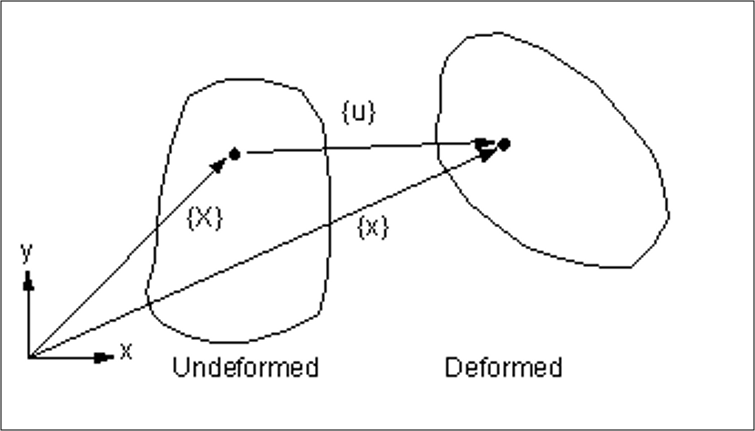
\includegraphics[width=0.7\linewidth]{deformovane-nedeformovane-souradnice}
	\caption{Souřadnice}
	\label{fig:deformovane-nedeformovane-souradnice}
\end{figure}

\section{Tenzory deformace}
% !TeX root = skripta-konstitutivni-vztahy.tex
% !TeX lastmodified = 2017-10-19

\subsection{Cauchy-Greenův tenzor deformace}
Tato definice nepracuje s~přetvořeními, ale s~poměrnými protaženími, podobně jako tenzor deformačního gradientu $\bm{F}$, z~nějž se odvozuje pomocí vztahů:

Pravý Cauchy-Greenův tenzor deformace
\begin{equation}
	\bm{C} = \bm{F}^T \bm{F}
	\quad\Leftrightarrow\quad
	C_{ij} = F_{ki} F_{kj}
\end{equation}
Levý Cauchy-Greenův tenzor deformace
\begin{equation}
	\bm{B} = \bm{F} \bm{F}^T
	\quad\Leftrightarrow\quad
	B_{ij} = F_{ik} F_{jk}
\end{equation}

Hlavními souřadnicemi tohoto tenzoru jsou kvadráty poměrných protažení v~hlavních směrech
\begin{equation}
	\bm{C} = \left(\begin{matrix}
		\lambda_1^2 & 0 & 0\\
		0 & \lambda_2^2 & 0\\
		0 & 0 & \lambda_3^2
	\end{matrix}\right)
\end{equation}

\subsubsection{Invarianty Cauchy-Greenova tenzoru deformace}
Invarianty tohoto tenzoru lze v hlavním souřadnicovém systému vyjádřit následovně:
\begin{align}
	I_1 &= \lambda_1^2 + \lambda_2^2 + \lambda_3^2\\
	I_2 &= \lambda_1^2 \lambda_2^2 + \lambda_2^2 \lambda_3^2 + \lambda_3^2 \lambda_1^2\\
	I_3 &= \lambda_1^2 \lambda_2^2 \lambda_3^2 = J^2
\end{align}

Zde $J$ je třetí invariant tenzoru deformačního gradientu. Třetí invariant tedy i~u~Cauchy-Greenova tenzoru deformace vyjadřuje změnu objemu (je roven jedné, pokud se při deformaci objem nemění).

Tenzorový zápis těchto invariantů je následující
\footnote{*G.A.Holzapfel:Nonlinear solid mechanics. Wiley, 2001, p. 25.}
\begin{align}
	I_1 &= \mathrm{Sp}(\bm{C})%todo zarovnání
	&\quad\Leftrightarrow\quad
	I_1 &= C_{ii}\\
	I_2 &= \frac{1}{2} \left[\mathrm{Sp}(\bm{C})^2 - \mathrm{Sp}(\bm{C}^2)\right]
	&\quad\Leftrightarrow\quad
	I_2 &= \frac{1}{2} (C_{ii} C_{jj} - C_{ij} C_{ji})\\
	I_3 &= \det(\bm{C})
\end{align}

%\subsubsection{Modifikované invarianty Cauchy-Greenova tenzoru deformace}
%Ve vztazích pro funkce měrné energie napjatosti se obvykle používají tzv. modifikované hodnoty hlavních poměrných protažení, které vyjadřují pouze tvarovou (deviátorovou) část tenzoru deformace, a~z~nich odvozené modifikované invarianty Cauchy-Greenova tenzoru deformace:
%\begin{align}
%	\bar{I}_1 &= \bar{\lambda}_1^2 + \bar{\lambda}_2^2 + \bar{\lambda}_3^2\\
%	\bar{I}_2 &= \bar{\lambda}_1^2 \bar{\lambda}_2^2 +\bar{ \lambda}_2^2 \bar{\lambda}_3^2 + \bar{\lambda}_3^2 \bar{\lambda_1}^2\\
%	I_3 &= \bar{\lambda}_1^2 \bar{\lambda}_2^2 \bar{\lambda}_3^2 = 1
%\end{align}

\subsubsection{Modifikované invarianty Cauchy-Greenova tenzoru deformace}
Modifikované (též někdy označované jako redukované) invarianty Cauchy-Greenova tenzoru deformace se ve vztazích pro funkce měrné energie napjatosti používají pro popis deviátorové složky deformace. Tak jako deviátor tenzoru malých přetvoření vznikl odečtením středního přetvoření od jednotlivých složek délkových přetvoření, zde dostaneme příslušná poměrná protažení dělením jednotlivých složek středním protažením $\lambda_s$. 

Pak dostaneme modifikovaná hlavní protažení z~rovnice
\begin{equation}
\bar{\lambda}_p = J^{-\frac{1}{3}} \lambda_p \quad (p = 1,2,3)
\end{equation}

Modifikované invarianty Cauchy-Greenova tenzoru deformace jsou pak dány
\begin{align}
\bar{I}_1
&= \bar{\lambda}_1^2 + \bar{\lambda}_2^2 + \bar{\lambda}_3^2
= \left(\lambda_1^2 + \lambda_2^2 + \lambda_3^2\right) J^{-\frac{2}{3}}
= I_1 J^{-\frac{2}{3}}
= I_1 I_3^{-\frac{1}{3}}\\
\bar{I}_2
&= \bar{\lambda}_1^2 \bar{\lambda}_2^2 + \bar{\lambda}_2^2 \bar{\lambda}_3^2 + \bar{\lambda}_1^2 \bar{\lambda}_3^2
= \left(\lambda_1^2 \lambda_2^2 + \lambda_2^2 \lambda_3^2 + \lambda_1^2 \lambda_3^2\right) J^{-\frac{4}{3}}
= I_2 J^{-\frac{4}{3}}
= I_2 I_3^{-\frac{2}{3}}
\end{align}

% !TeX root = skripta-konstitutivni-vztahy.tex
% !TeX lastmodified = 2014-11-10

\subsection{Tenzor deformačního gradientu}
Složkami tenzoru deformačního gradientu $\bm{F}$ jsou poměrná protažení
\begin{equation}
	\lambda_x  = \frac{\partial x}{\partial X}
	\qquad
	\lambda_y  = \frac{\partial y}{\partial Y}
	\qquad
	\lambda_z  = \frac{\partial z}{\partial Z}
\end{equation}

Obecně je lze zapsat ve tvaru
\begin{equation}
	\lambda_{ij}  = \frac{\partial x_i}{\partial X_j}
\end{equation}

Úplný maticový zápis v obecném souřadnicovém systému je
\begin{equation}
	\bm{F} = \left(\begin{matrix}
		\frac{\partial x_1}{\partial X_1} & \frac{\partial x_1}{\partial X_2} & \frac{\partial x_1}{\partial X_3}\\
		\frac{\partial x_2}{\partial X_1} & \frac{\partial x_2}{\partial X_2} & \frac{\partial x_2}{\partial X_3}\\
		\frac{\partial x_3}{\partial X_1} & \frac{\partial x_3}{\partial X_2} & \frac{\partial x_3}{\partial X_3}
	\end{matrix}\right)
\end{equation}

Třetí invariant tenzoru deformačního gradientu je dán determinantem této matice $\bm{F}$, který lze nejsnáze určit z~hlavních hodnot poměrných protažení pomocí vztahu
\begin{equation}
	J = \det(\bm{F}) = \lambda_1 \lambda_2 \lambda_3
\end{equation}

\subsubsection{Vlastnosti tenzoru deformačního gradientu}
Tenzor deformačního gradientu je obecně nesymetrický, v~důsledku toho existují dva v~principu odlišné Cauchy-Greenovy tenzory deformace (levý a~pravý).

Třetí invariant $J$ tenzoru deformačního gradientu $\bm{F}$ udává poměrnou objemovou změnu elementu, jak plyne z následujícího vztahu: 
\begin{equation}
	e
	= \frac{V_\text{def} - V_\text{nedef}}{V_\text{nedef}}
	= \frac{\diff x \diff y \diff z - \diff X \diff Y \diff Z}{\diff X \diff Y \diff Z}
	= \frac{\partial x}{\partial X} \frac{\partial y}{\partial Y} \frac{\partial z}{\partial Z} - 1
	= \lambda_1 \lambda_2 \lambda_3 -1
	= J - 1
\end{equation}

Jako každý tenzor lze i~tenzor deformačního gradientu tedy rozložit na část kulovou (změna objemu) a~deviátorovou (změna tvaru). 

U~smluvních přetvoření byla kulová část tenzoru dána aritmetickým průměrem hlavních přetvoření. Podobně zde je kulová část dána průměrem hlavních souřadnic tenzoru, ovšem nikoli aritmetickým, nýbrž geometrickým, protože změna objemu je dána součinem těchto souřadnic.

Pro střední protažení platí tedy
\begin{equation}
	\lambda_s
	= \sqrt[3]{\lambda_1 \lambda_2 \lambda_3}
	= \sqrt[3]{J}
	= J^{\frac{1}{3}}
\end{equation}




% !TeX root = skripta-konstitutivni-vztahy-materialu.tex
% !TeX lastmodified = 2019-11-27

\subsection{Tenzor protažení (stretch tensor)}
I~v~nedeformovaném stavu elementu může mít matice definující tenzor deformačního gradientu $\bm{F}$ složky odlišné od jednotkové matice; je to dáno případnou rotací elementu v~důsledku velkých deformací tělesa.  Polární dekompozicí tenzoru $\bm{F}$ lze tento rozložit na tenzor rotace $\bm{R}$ (vyjadřující rotaci tuhého tělesa) a~tenzor protažení $\bm{U}$ nebo $\bm{V}$ (popisující deformaci tělesa). Tento tenzor je již symetrický a~energeticky konjugovaný se symetrickou částí Biotova tenzoru napětí $\bm{T_B}$. 

Tenzor deformačního gradientu je definován vztahem
\begin{equation}
	F_{iJ} := \frac{\partial x_i}{\partial X_J}
\end{equation}
který můžeme přepsat do maticové podoby s~konečnými diferencemi namísto derivací
\begin{equation}
	\bm{F} = \frac{\Delta \bm{x}}{\Delta \bm{X}}
\end{equation}

Polární dekompozice tenzoru $\bm{F}$ pak spočívá v~jeho rozložení na tenzor 
rotace $\bm{R}$ a~pravý nebo levý tenzor protažení (stretch tensor) $\bm{U}$ nebo $\bm{V}$:
\begin{equation}
	\bm{F} = \bm{R} \bm{U} = \bm{V} \bm{R}
	\quad\Rightarrow\quad
	\bm{U} = \bm{R}^{-1} \bm{F} = \bm{R}^T \bm{F};
	\quad
	\bm{V} = \bm{F} \bm{R}^{-1} = \bm{F} \bm{R}^T
\end{equation}
Zde se využívá ortogonality tenzoru rotace $\bm{R}$, pro který tedy inverzní matice se rovná matici transponované.

Tenzor rotace $\bm{R}$ je v rovině (2D zjednodušení) definován vztahem
\begin{equation}
	\bm{R} = \left(\begin{matrix}
		\cos(\psi) & \sin(\psi)\\
		-\sin(\psi) & \cos(\psi)\\
	\end{matrix}\right),
\end{equation}
kde úhel $\psi$ lze určit ze složek tenzoru deformačního gradientu pomocí vztahu
\begin{equation}
	\psi = \arctan\left(\frac{F_{12} - F_{21}}{F_{11} + F_{22}}\right)
\end{equation}

Pomocí tenzorů protažení $\bm{U}$ a~$\bm{V}$ lze pak definovat také Cauchyho-Greenův tenzor deformace $C$ a~Fingerův tenzor deformace $\bm{B}$ pomocí vztahů:
\begin{equation}
	\bm{C} = \bm{F}^T \bm{F} = \bm{U}^T \bm{U} = U^2; \quad
	\bm{B} = \bm{F} \bm{F}^T = \bm{V} \bm{V}^T = V^2; \quad
\end{equation}
Zde se navíc využívá faktu, že oba tyto tenzory jsou (na rozdíl od tenzoru deformačního gradientu $\bm{F}$) vždy symetrické. Hlavní složky tenzoru $\bm{U}$ i~$\bm{V}$ jsou stejné a představují hlavní poměrná protažení (principal stretches). 

\section{Tenzory přetvoření}
% !TeX root = skripta-konstitutivni-vztahy.tex
% !TeX lastmodified = 2006-11-04

\begin{figure}[H]
	\centering
	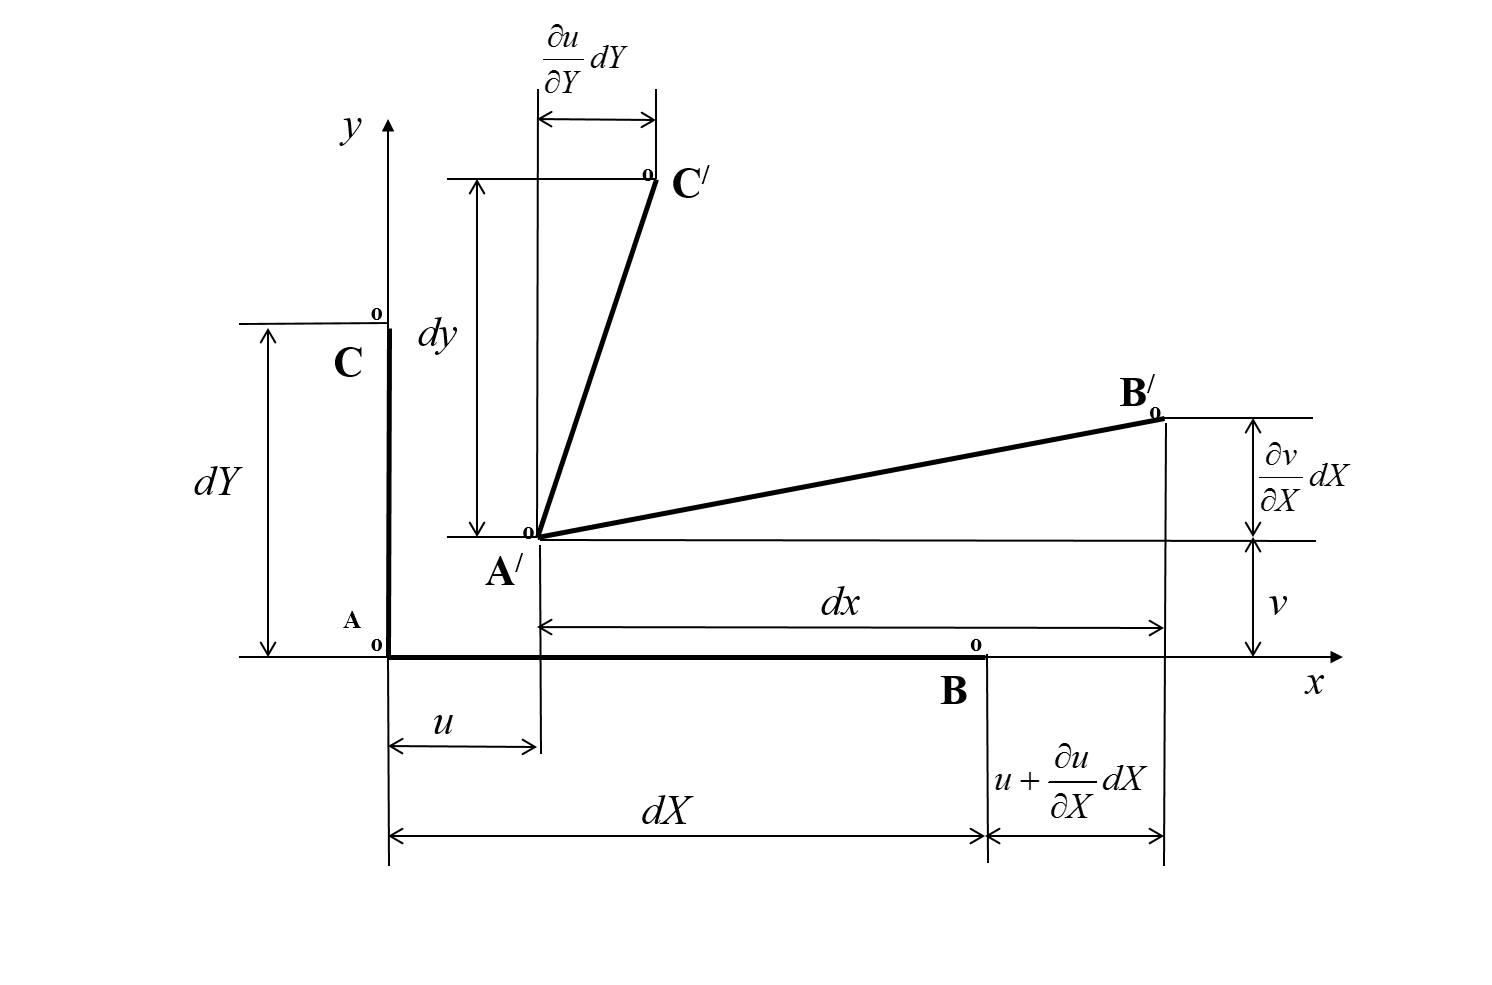
\includegraphics[width=0.7\linewidth]{pretvoreni}
	\caption{Přetvoření}
	\label{fig:pretvoreni}
\end{figure}

% !TeX root = skripta-konstitutivni-vztahy.tex
% !TeX lastmodified = 2006-11-05

\subsection{Tenzor smluvního přetvoření (pro malé deformace)}
Délková (označení viz obrázek \ref{fig:pretvoreni}):
\begin{equation}
	\varepsilon_x
	= \frac{\diff x - \diff X}{\diff X}
	= \frac{\diff X + u + \frac{\partial u}{\partial X}\diff X - u - \diff X}{\diff X}
	= \frac{\partial u}{\partial X}
\end{equation}

Pro ostatní složky analogicky:
\begin{equation}
	\varepsilon_x
	= \frac{\partial v}{\partial Y}
	\qquad
	\varepsilon_z
	= \frac{\partial w}{\partial Z}
\end{equation}

Úhlová (zkosy):
\begin{equation}
	\gamma_{xy}
	= \gamma_{AB} + \gamma_{AC}
	= \tan(\gamma_{AB}) + \tan(\gamma_{AB})
	= \frac{\frac{\partial v}{\partial X} \diff X}{\diff X}
	+ \frac{\frac{\partial u}{\partial Y} \diff Y}{\diff Y}
	= \frac{\partial v}{\partial X} + \frac{\partial u}{\partial Y}
\end{equation}

Pro ostatní složky analogicky:
\begin{equation}
	\gamma_{yz}
	= \frac{\partial v}{\partial Z} + \frac{\partial w}{\partial Y}
	\qquad
	\gamma_{xz}
	= \frac{\partial u}{\partial Z} + \frac{\partial w}{\partial X}
\end{equation}

Vzhledem k tomu, že složkami tenzoru přetvoření jsou poloviční zkosy, lze napsat obecný tenzorový vztah
\begin{equation}
	\bm{\varepsilon} := \tfrac{1}{2} \left( \nabla\bm{u} + \nabla^T\bm{u} \right)
	\quad\Leftrightarrow\quad
	\varepsilon_{ij} := \frac{1}{2} \left( \frac{\partial u_i}{\partial X_j} + \frac{\partial u_j}{\partial X_i} \right),
\end{equation}
kde souřadnicím $X$, $Y$, $Z$ odpovídají $X_i$ a~posuvům $u$, $v$, $w$ posuvy $u_i$ (pro $i=1,2,3$).

% !TeX root = skripta-konstitutivni-vztahy.tex
% !TeX lastmodified = 2019-10-23

\subsection{Tenzor Greenova-Lagrangeova přetvoření}\label{sec:green-lagrange}
Přetvoření (poměrná deformace) je rovněž vztažena k původním (nedeformovaným) rozměrům, ale je respektováno i natáčení elementu. Pak je délkové přetvoření (označení viz obrázek \ref{fig:pretvoreni}):
\begin{equation}\begin{split}
	E^L_x &= \frac{A'B' - AB}{AB}
	= \frac{\sqrt{\diff x^2 + \left( \frac{\partial v}{\partial X} \diff X \right)^2 + \left( \frac{\partial w}{\partial X} \diff X \right)^2} - \diff X}{\diff X}\\
	&= \frac{\sqrt{ \left( \diff X + u + \frac{\partial u}{\partial X} \diff X - u \right)^2 + \left( \frac{\partial v}{\partial X} \diff X \right)^2 + \left( \frac{\partial w}{\partial X} \diff X \right)^2} - \diff X}{\diff X}
\end{split}\end{equation}

Deformovaná délka elementu dx se zde počítá aplikací Pythagorovy věty ve 3D prostoru (není v obrázku zakresleno). Pro zjednodušení vztahu použijeme první dva členy binomické řady:
\begin{equation}
	\sqrt{1 + \kappa} = 1 + \frac{\kappa}{2} - \frac{\kappa^2}{8} + \frac{\kappa^3}{16} - \ldots
\end{equation}
Pak dostaneme:
\begin{equation}\begin{split}
	E^L_x
	&= \frac{\diff X \sqrt{ 1 + 2 \frac{\partial u}{\partial X} + \left( \frac{\partial u}{\partial X} \right)^2 + \left( \frac{\partial v}{\partial X} \right)^2 + \left( \frac{\partial w}{\partial X} \right)^2} - \diff X}{\diff X}\\
	&= 1 + \frac{2 \frac{\partial u}{\partial X} + \left( \frac{\partial u}{\partial X} \right)^2 + \left( \frac{\partial v}{\partial X} \right)^2 + \left( \frac{\partial w}{\partial X} \right)^2}{2} - 1\\
	&= \frac{\partial u}{\partial X} + \frac{1}{2} \left[ \left( \frac{\partial u}{\partial X} \right)^2 + \left( \frac{\partial v}{\partial X} \right)^2 + \left( \frac{\partial w}{\partial X} \right)^2 \right]
\end{split}\end{equation}
Pro ostatní složky délkových přetvoření platí analogicky:
\begin{equation}\begin{split}
	E^L_y
	&= \frac{\partial v}{\partial Y} + \frac{1}{2} \left[ \left( \frac{\partial u}{\partial Y} \right)^2 + \left( \frac{\partial v}{\partial Y} \right)^2 + \left( \frac{\partial w}{\partial Y} \right)^2 \right]\\
	E^L_z
	&= \frac{\partial w}{\partial Z} + \frac{1}{2} \left[ \left( \frac{\partial u}{\partial Z} \right)^2 + \left( \frac{\partial v}{\partial Z} \right)^2 + \left( \frac{\partial w}{\partial Z} \right)^2 \right]
\end{split}\end{equation}

Zobecnění na všechny složky tenzoru přetvoření je možné pomocí tenzorového zápisu
\begin{equation}
	E^L_{ij}
	= \frac{1}{2} \left[ \frac{\partial u_i}{\partial X_j} + \frac{\partial u_j}{\partial X_i} + \frac{\partial u_k}{\partial X_j} \frac{\partial u_k}{\partial X_i} \right]
\end{equation}
Tento zápis používá Einsteinovo sčítací pravidlo.

% !TeX root = skripta-konstitutivni-vztahy.tex
% !TeX lastmodified = 2019-10-23

\subsection{Tenzor Almansiho-Hamelova přetvoření}
Podle Almansiho se poměrné přetvoření vztahuje ke konečným (nedeformovaným) rozměrům. Pak délkové přetvoření lze vyjádřit (označení viz obrázek \ref{fig:pretvoreni}):
\begin{equation}
	E^A_x = \frac{A'B' - AB}{A'B'}
\end{equation}

Podobným postupem jako pro tenzor Greenova-Lagrangeova přetvoření se dospěje k obecnému tenzorovému zápisu ve tvaru:
\begin{equation}
	E^A_{ij}
	= \frac{1}{2} \left[ \frac{\partial u_i}{\partial x_j} + \frac{\partial u_j}{\partial x_i} - \frac{\partial u_k}{\partial x_j} \frac{\partial u_k}{\partial x_i} \right]
\end{equation}
Také tento zápis používá Einsteinovo sčítací pravidlo.

Praktické použití tohoto tenzoru je omezeno tím, že konečné (deformované) souřadnice obvykle předem neznáme.

% !TeX root = skripta-konstitutivni-vztahy.tex
% !TeX lastmodified = 2016-10-10

\subsection{Cauchyho (logaritmický) tenzor přetvoření}
Nedostatky tenzorů konečných přetvoření:
\begin{itemize}
	\item Green-Lagrange: změny délek jsou stále vztahovány k~původním hodnotám, zatímco aktuální již mohou být v průběhu procesu zatěžování významně odlišné.
	\item Almansi-Hamel: změny délek jsou stále vztahovány ke konečným (deformovaným) hodnotám délek, zatímco aktuální od nich mohou být v~průběhu procesu zatěžování ještě podstatně odlišné.
\end{itemize}

Cauchyho definice přetvoření je exaktnější v~tom, že infinitezimální přírůstek délky vztahuje vždy k~aktuální délce v~daném stádiu zatěžovacího procesu.

Přetvoření úsečky o~původní délce $X_{i0}$, která se vlivem zatížení mění na aktuální hodnotu $X_i$ až dosáhne konečné (deformované) délky $x_{ik}$, určíme integrací přírůstků její délky $\diff x_i$:
\begin{equation}
	E^C_{ij}
	= \int\limits_{X_{i0}}^{x_{ik}} \frac{1}{x_i} \diff x_i
	= \left. \ln(x) \right\rvert_{X_{i0}}^{x_{ik}}
	= \ln(x_{ik}) - \ln(X_{i0})
	= \ln\left(\frac{x_{ik}}{X_{i0}}\right)
	= \ln(\lambda_i)
\end{equation}

\subsubsection{Tenzorová formulace Cauchyho tenzoru přetvoření}

Složky tohoto tenzoru jsou rovny přirozeným logaritmům odpovídajících složek tenzoru deformačního gradientu.


Souřadnice tohoto tenzoru jsou tedy rovny přirozeným logaritmům odpovídajících souřadnic tenzoru deformačního gradientu.
\begin{equation}
	E^C_{ij} = \ln(F_{ij}) = \frac{1}{2} \ln(C_{ij})
\end{equation}

% !TeX root = skripta-konstitutivni-vztahy.tex
% !TeX lastmodified = 2016-12-06

\subsection{Vzájemné přepočtové vztahy pro tenzory přetvoření}
Nejvhodnější pro vzájemný přepočet tenzorů přetvoření jsou poměrná protažení $\lambda_i$, tedy složky tenzoru deformačního gradientu. Pro jednoduchost jsou uvedena jen hlavní přetvoření jako funkce hlavních poměrných protažení $\lambda_i$:

Smluvní přetvoření -- vztah se odvozuje v~základní PP: 
\begin{equation}
	\varepsilon_i = \lambda_i - 1
\end{equation}

Green-Lagrange:
\begin{equation}
	E^L_i
	= \frac{\partial u_i}{\partial X_i} + \frac{1}{2} \left(\frac{\partial u_i}{\partial X_i}\right)^2
	= \lambda_i - 1 + \frac{1}{2} (\lambda_i - 1)^2
	= \frac{1}{2} (\lambda_i^2 - 1)
\end{equation}
příp. v~maticovém vyjádření:
\begin{equation}
	\bm{E}^L = \frac{1}{2} \left(\bm{F}^T \bm{F} - \bm{1}\right)
\end{equation}

Almansi-Hamel:
\begin{equation}
	E^A_i
	= \frac{\partial u_i}{\partial x_i} - \frac{1}{2} \left(\frac{\partial u_i}{\partial x_i}\right)^2
	= 1 - \lambda_i^{-1} - \frac{1}{2} (1 - \lambda_i^{-1})^2
	= \frac{1}{2} (1 - \lambda_i^{-2})
\end{equation}

Cauchy:
\begin{equation}
	E^C_i = \ln(\lambda_i)
\end{equation}

\subsubsection{Rozdíly mezi jednotlivými definicemi tenzoru přetvoření}
\begin{figure}[H]
	\centering
	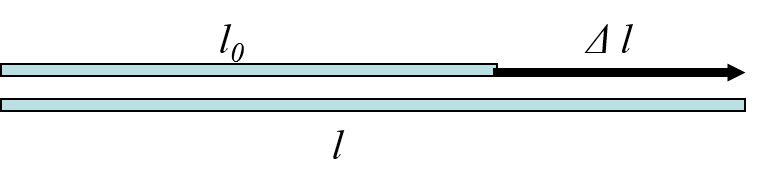
\includegraphics{1d-pretvoreni}
	\caption{Protažení tyče}
	\label{fig:1d-pretvoreni}
\end{figure}

\begin{align}
	E^L &= \frac{1}{2} \frac{l^2 - l_0^2}{l_0^2} = \frac{1}{2} (\lambda^2 - 1)\\
	E^A &= \frac{1}{2} \frac{l^2 - l_0^2}{l^2} = \frac{1}{2} (1 - \lambda^{-2})\\
	\varepsilon &= \frac{l - l_0}{l_0} = \lambda - 1\\
	E^C &= \ln\left(\frac{l}{l_0}\right) = \ln(\lambda)
\end{align}
% Doplnil bych graf v tlaku a řekl které jsou konečné

\begin{figure}[H]
	\centering
	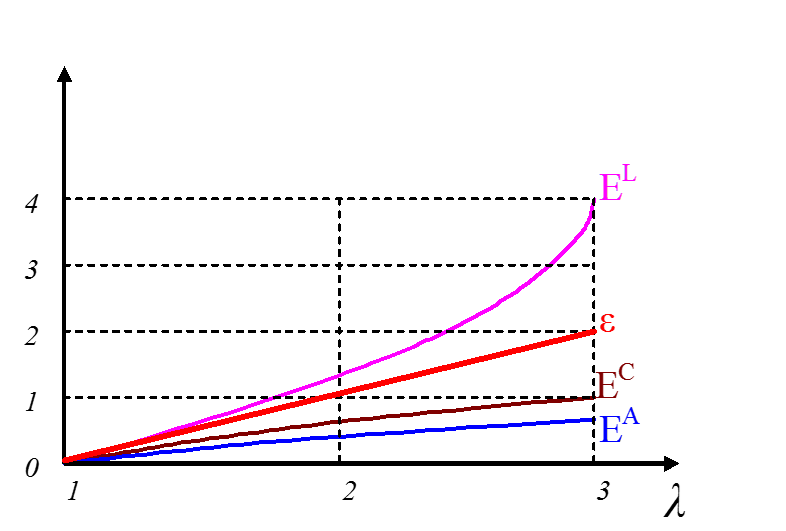
\includegraphics{Obrazky/tenzory-pretvoreni}
	\caption{Přetvoření v tahu}
	\label{fig:tenzory-pretvoreni}
\end{figure}

\section{Tenzory napětí}
% !TeX root = skripta-konstitutivni-vztahy.tex
% !TeX lastmodified = 2019-10-23

\subsection{Tenzor Cauchyho napětí}
Tenzor Cauchyho napětí (v praxi často skutečná napětí -- true stress) je definován jako skutečná elementární síla vztažená na skutečnou (tj. deformovanou) plochu elementu podle vztahu (platí pro hlavní napětí):
\begin{equation}
	\sigma_i = \frac{\diff F_i}{\diff x_j \diff x_k}
\end{equation}
Konkrétně pro hlavní napětí ve směru 1 platí:
\begin{equation}
	\sigma_1 = \frac{\diff F_1}{\diff x_2 \diff x_3}
\end{equation}

% !TeX root = skripta-konstitutivni-vztahy.tex
% !TeX lastmodified = 2006-11-06

\subsection{Piola-Kirchhoffův tenzor napětí 1.~druhu}
1.~Piola-Kirchhoffův tenzor napětí (označovaný také jako Lagrangeův nebo Piolův, v~praxi často smluvní napětí -- engineering stress) je definován jako skutečná elementární síla vztažená na původní (tj. nedeformovanou) plochu elementu podle vztahu (platí pro hlavní napětí):
\begin{equation}
	\tau_i = \frac{\diff F_i}{\diff X_j \diff X_k}
\end{equation}
Konkrétně pro hlavní napětí ve směru 1 platí:
\begin{equation}
	\tau_1 = \frac{\diff F_1}{\diff X_2 \diff X_3}
\end{equation}

% !TeX root = skripta-konstitutivni-vztahy.tex
% !TeX lastmodified = 2010-03-16

\subsection{Piola-Kirchhoffův tenzor napětí 2.~druhu}
2.~Piola-Kirchhoffův (označovaný také jen jako Kirchhoffův) tenzor napětí je definován jako elementární síla $\diff F_{0i}$ vztažená na původní (tj. nedeformovanou) plochu elementu. Tato síla je však při přenášení na původní element změněna oproti skutečné síle $\diff F_i$ stejným poměrem jako elementární rozměr v~odpovídajícím směru. Ten se mění při zatížení podle vztahu
\begin{equation}
	\diff x_i = \frac{\partial x_i}{\partial X_i} \diff X_i,
\end{equation}
resp. při zpětné transformaci do nedeformovaného tvaru
\begin{equation}
	\diff X_i = \frac{\partial X_i}{\partial x_i} \diff x_i.
\end{equation}

Podobně transformujeme i~elementární sílu
\begin{equation}
	\diff F_{0i} = \frac{\partial X_i}{\partial x_i} \diff F_i,
\end{equation}
takže  napětí je
\begin{equation}
	S_i = \frac{\diff F_{0i}}{\diff X_j \diff X_k}
\end{equation}
Konkrétně pro normálové napětí ve směru 1 platí:
\begin{equation}
	S_i = \frac{\diff F_{01}}{\diff X_2 \diff X_3}
	= \frac{\frac{\partial X_1}{\partial x_1} \diff F_1}{\diff X_2 \diff X_3}
\end{equation}

Tento tenzor nemá jasný fyzikální význam, používá se proto, že je i~pro velká přetvoření symetrický a~je energeticky konjugovaný s~Green-Lagrangeovým tenzorem přetvoření.

% !TeX root = skripta-konstitutivni-vztahy.tex
% !TeX lastmodified = 2010-03-16

\subsection{Vzájemné přepočtové vztahy pro tenzory napětí}
Nejvhodnější pro vzájemný přepočet tenzorů přetvoření jsou poměrná protažení $\lambda_i$, tedy složky tenzoru deformačního gradientu. V~hlavním souřadnicovém systému platí následující vztahy:

Hlavní Cauchyho (skutečné) napětí lze vyjádřit pomocí 1.P.K. napětí
\begin{equation}
	\sigma_i = \frac{\diff F_i}{\diff x_j \diff x_k}
	= \frac{\diff F_i}{\lambda_j \diff X_j \lambda_k \diff X_k}
	= \frac{\tau_i}{\lambda_j \lambda_k}
\end{equation}

Pro nestlačitelný materiál platí $\lambda_i\lambda_j\lambda_k=1$ a~tedy napětí jsou ve vztahu
\begin{equation}
	\sigma_i = \frac{\tau_i}{\lambda_j \lambda_k} = \tau_i \lambda_i
\end{equation}

Podobně lze vyjádřit 2.P.K. napětí
\begin{equation}
	S_i = \frac{\diff F_{0i}}{\diff X_j \diff X_k}
	= \frac{\frac{\partial X_i}{\partial x_i} \diff F_i}{\diff X_j \diff X_k}
	= \frac{\frac{1}{\lambda_i} \diff F_i}{\diff X_j \diff X_k}
	= \frac{1}{\lambda_i} \tau_i
\end{equation}

Cauchyho napětí lze vyjádřit i~pomocí 2.P.K. napětí
\begin{equation}
	\sigma_i = \frac{\tau_i}{\lambda_j \lambda_k}
	= \frac{\lambda_i}{\lambda_j \lambda_k} S_i,
\end{equation}
nebo jednodušeji pro nestlačitelný materiál
\begin{equation}
	\sigma_i = \lambda_i \tau_i = \lambda_i^2 S_i.
\end{equation}

% !TeX root = skripta-konstitutivni-vztahy.tex
% !TeX lastmodified = 2018-11-13

\subsection{Energeticky konjugované tenzory}
Pro správné (jednoznačné) určení energie napjatosti je nutné pracovat se vzájemně si odpovídajícími tenzory napětí a~přetvoření.
Těmto dvojicím tenzorů říkáme energeticky konjugované tenzory.
Jsou to tedy vzájemně přiřazené dvojice tenzorů napětí a~přetvoření, jejichž vzájemnou kombinací lze dostat (i~v~případě velkých přetvoření a~velkých posuvů) energii napjatosti.

Takto konjugované jsou např.
\begin{itemize}
	\item Green-Lagrangeův tenzor přetvoření a~2.~Piola-Kirchhoffův tenzor napětí,
	\item pravý Cauchy-Greenův tenzor deformace a~2.~Piola-Kirchhoffův tenzor napětí,
	\item tenzor protažení $\bm{U}$ (pravý) a~Biotův tenzor napětí $\bm{T}_B$ (symetrický, v~těchto oporách není popsán),
	\item tenzor deformace daný vztahem $\bm{F} - \bm{1}$ (jednotkový tenzor) a~1.~Piola-Kirchhoffův tenzor napětí.
\end{itemize}

%% !TeX root = skripta-konstitutivni-vztahy.tex
% !TeX lastmodified = 2010-03-16

\subsection{Modifikované invarianty Cauchy-Greenova tenzoru deformace}
Modifikované (též někdy označované jako redukované) invarianty Cauchy-Greenova tenzoru deformace se používají pro popis deviátorové složky deformace. Tak jako deviátor tenzoru malých přetvoření vznikl odečtením středního přetvoření od jednotlivých složek délkových přetvoření, zde dostaneme příslušná poměrná protažení dělením jednotlivých složek středním protažením $\lambda_s$. 

Pak dostaneme modifikovaná hlavní protažení z~rovnice
\begin{equation}
	\bar{\lambda}_p = J^{-\frac{1}{3}} \lambda_p \quad (p = 1,2,3)
\end{equation}

Modifikované invarianty Cauchy-Greenova tenzoru deformace jsou pak dány 
\begin{align}
	\bar{I}_1
	&= \bar{\lambda}_1^2 + \bar{\lambda}_2^2 + \bar{\lambda}_3^2
	= \left(\lambda_1^2 + \lambda_2^2 + \lambda_3^2\right) J^{-\frac{2}{3}}
	= I_1 J^{-\frac{2}{3}}
	= I_1 I_3^{-\frac{1}{3}}\\
	\bar{I}_2
	&= \bar{\lambda}_1^2 \bar{\lambda}_2^2 + \bar{\lambda}_2^2 \bar{\lambda}_3^2 + \bar{\lambda}_1^2 \bar{\lambda}_3^2
	= \left(\lambda_1^2 \lambda_2^2 + \lambda_2^2 \lambda_3^2 + \lambda_1^2 \lambda_3^2\right) J^{-\frac{4}{3}}
	= I_2 J^{-\frac{4}{3}}
	= I_2 I_3^{-\frac{2}{3}}
\end{align}

% !TeX root = skripta-konstitutivni-vztahy.tex
% !TeX lastmodified = 2018-11-20

\subsection{(Pseudo)invarianty pravého Cauchy-Greenova tenzoru deformace}
Vztahují se pouze k~deviátorové složce měrné energie napjatosti materiálu, protože vzhledem k~předpokladu nulového průměru vláken a~tedy jejich nulovému objemu nemohou vlákna ovlivňovat volumetrickou složku energie napjatosti.
Byly zavedeny pro popis deformace vláken v~závislosti na pravém Cauchy-Greenově deformačním tenzoru a~směrových vektorech $\bm{a}$ nebo $\bm{b}$, příp. směrových tenzorech (nazývaných  také „structural tensors“) $\bm{A}$ nebo $\bm{B}$ vláken, definovaných vztahem:
\begin{equation*}
\bm{A} = \bm{a} \otimes \bm{a}
\quad\Leftrightarrow\quad
A_{ij} = a_i a_j
\end{equation*}

Samotné (pseudo)invarianty jsou definovány následujícími vztahy:
\begin{align*}
\bar{I}_4 &= \bar{\bm{C}} : \bm{A} = \bm{a} \cdot \bar{\bm{C}} \bm{a} \quad&\Leftrightarrow\quad \bar{I}_4 &= a_i \bar{C}_{ij} a_j\\
\bar{I}_5 &= \bar{\bm{C}}^2 : \bm{A} = \bm{a} \cdot \bar{\bm{C}}^2 \bm{a} \quad&\Leftrightarrow\quad \bar{I}_5 &= a_i \bar{C}_{ij}^2 a_j\\
\bar{I}_6 &= \bar{\bm{C}} : \bm{B} = \bm{b} \cdot \bar{\bm{C}} \bm{b} \quad&\Leftrightarrow\quad \bar{I}_6 &= b_i \bar{C}_{ij} b_j\\
\bar{I}_7 &= \bar{\bm{C}}^2 : \bm{B} = \bm{b} \cdot \bar{\bm{C}}^2 \bm{b} \quad&\Leftrightarrow\quad \bar{I}_7 &= b_i \bar{C}_{ij}^2 b_j\\
\bar{I}_8 &= (\bm{a} \cdot \bm{b}) \bm{a} \cdot \bm{C} \bm{b} \quad&\Leftrightarrow\quad \bar{I}_8 &= (a_k b_k) a_i \bar{C}_{ij} b_j\\
\bar{I}_9 &= \zeta = (\bm{a} \cdot \bm{b})^2 \quad&\Leftrightarrow\quad \bar{I}_9 &= (a_i b_i)^2
\end{align*}

Dá se ukázat, že invarianty $\bar{I}_4$ a~$\bar{I}_6$ vyjadřují protažení jednotlivých osnov výztužných vláken, podobně jako invarianty vyššího stupně $\bar{I}_5$ a $\bar{I}_7$, zatímco $\bar{I}_8$ se vztahuje ke vzájemnému ovlivnění obou osnov vláken a $\bar{I}_9$ je pouze geometrická konstanta.
